\documentclass[12pt, letterpaper]{article}

\usepackage{amsmath}
\usepackage{amsfonts}
\usepackage{algorithm2e}
\usepackage{float}
\usepackage{subcaption}

\RestyleAlgo{ruled}

\usepackage{graphicx}
\graphicspath{ {./pics/} }

\title{Fisher-Kolmogorov equations for neurodegenerative diseases}
\author{Andrea Boin, Giacomo Pauletti, Lorenzo Pettenuzzo}
\date{}

\begin{document}
\maketitle
\pagebreak

\tableofcontents
\pagebreak

% TODO: make introduction more formal, cleaner and add something about the objective about experimental values for the simulation (alpha average grey/white matter, D isotropic,...)
\section{Introduction}
The objective of this project is to apply various numerical methods to solve the Fisher-Kolmogorov equations to reproduce the results of the paper \cite{diffusion-paper}. The Fisher-Kolmogorov equations can be used to effectively model the spread of misfolded proteins in the brain, a process associated with numerous neurodegenerative diseases.

\subsection{Fisher-Kolmogorov equation}
\[
\begin{cases}
\displaystyle \frac{\partial c}{\partial t} - \nabla \cdot (D \nabla c) - \alpha c(1 - c) = 0 & \text{in } \Omega\\
\displaystyle D \nabla c \cdot \mathbf{n} = 0 & \text{on } \partial \Omega\\
c(t=0)=c_0 & \text{in } \Omega
\end{cases}
\]
\begin{itemize}
    \item $c$: concentration of the misfolded protein in a region of the brain $(0\leq c\leq1)$
    \item $\alpha$: constant of concentration growth
    \item $D$: diffusion coefficient of the misfolded protein.\\
It can be isotropic (a scalar) or anisotropic (a square matrix).\\
In case of anisotropic coefficient the term can be computed as:

$$\underbar{D}=d^{\text{ext}}\underbar{I}+d^{\text{axn}}(\mathbf{n}\otimes\mathbf{n})$$

where $d^{\text{ext}}$ is the extracellular diffusion term, $d^{\text{axn}}$ is the axonal diffusion term and $\mathbf{n}$ the direction of axonal diffusion.

Usually extracellular diffusion is slower than axonal diffusion: $d^{\text{ext}}<d^{\text{axn}}$.

The Fisher-Kolmogorov equation is a \textbf{diffusion-reaction} equation with a nonlinear forcing term that can be used to model population growth. In this case it is used to model the spreading of proteins in the brain.

The interested problem is a \textbf{nonlinear parabolic PDE} with \textbf{Neumann boundary conditions}.
\end{itemize} 

\subsection{Mesh}
The mesh we used for the simulation is a 3D representation of a hemisphere of the human brain with 21211 points and 42450 cells.\\
To process the mesh with our software, we did convert the format from \textit{.stl} to \textit{.msh} using \textbf{GMSH} with the following procedure:
\begin{enumerate}
    \item Import the mesh (\textit{.stl}) in GMSH
    \item From the left menu, select "geometry $\rightarrow$ add $\rightarrow$ volume"
    \item Save the new generated \textit{.geo} file
    \item Define the 3D mesh: "mesh $\rightarrow$ define $\rightarrow$ 3D"
    \item Export the file as \textit{.msh}: "file $\rightarrow$ export $\rightarrow$ msh"
\end{enumerate}

\noindent The mesh isn't associated to any function that could provide information about axonal orientation so an anisotropic model can't be used to accurately simulate the evolution of the system.
\noindent Also there is no distinction between white and grey matter in the mesh. Different kinds of matter have different reaction coefficients so we used an average of the two for our simulations. 
\noindent We used an initial seed based on the function $$c(x,y,z,t=0)=\begin{cases}0.1&z<15\\-0.02z+0.4&15<z<20\\0&\text{otherwise}\end{cases}$$
\noindent The value 0.1 is the same value used in \cite{diffusion-paper}.
\noindent We used a decreasing ramp to avoid a step function as initial condition and obtain a continuous function.
%TODO: make mathematical part cleaner with a better logic order
%TODO: make sure math is correct and define a better notation
\subsection{Weak formulation and semi-discretized formulation}
By choosing a domain $V=H^1=\{v\in L^2|\nabla v\in L^2\}$ and considering a time domain $(0, T)$, the weak formulation of the problem is:

\vspace{1em}
\noindent Find $c(t)\in V$ such that $\forall v\in V$ and $\forall t\in(0,T)$:
$$\begin{cases}\int_\Omega\frac{\delta c}{\delta t}vd\Omega+\int_\Omega D\nabla c\nabla vd\Omega-\int_\Omega\alpha c(1-c)vd\Omega=0\\c(t=0)=c_0\end{cases}$$

\vspace{1em}
\noindent By renaming:
\begin{itemize}
    \item $d(c,v)=\int_\Omega D\nabla c\nabla vd\Omega$
    \item $e(c,v)=-\int_\Omega\alpha c(1-c)vd\Omega$
\end{itemize}

\noindent By introducing a triangulation $T_h=\{K|\Omega=\bigcup K\}$ of the domain $\Omega$ and defining with it a polynomial space $$X_h=\{v_h\in C^0(\bar\Omega)|v_{h|k}\in\mathbb{P}^r(K),\forall K\in T_h\}$$ we can obtain the discrete space $V_h=V\cap X_h$ for our discrete formulation.

\noindent The semi-discrete formulation can then be written as:

\vspace{1em}
\noindent
For each $t\in(0,T]$ find $c_h\in V_h$ such that:

\notag \begin{gather}
\int_\Omega\frac{\delta c_h}{\delta t}v_hd\Omega+d(c_h,v_h)+e(c_h,v_h)=0    
\qquad \forall v_h\in V_h
\end{gather}

\noindent given that $c_h(t=0)=c_{h,0}$

\section{Methods}

We studied the problem with 3 methods and implemented 2 of them algorithmically:
\begin{itemize}
    \item An \textbf{explicit} scheme in which all terms have been treated explicitly to handle the nonlinear part of the model.
    \item A \textbf{mixed explicit/implicit} scheme in which the linear terms have been treated implicitly while the nonlinear terms explicitly to get rid of nonlinarities.
    \item An \textbf{implicit} scheme in which all terms in the equation have been treated implicitly, and then the nonlinear parts have been solved with the Newton method.
\end{itemize}

\noindent To obtain a full discretization of the problem we need to partition the time domain in $N$ partitions of size $\Delta t$, obtaining $(0, T)=(0,N\Delta t)=\bigcup_{n=1}^N(t^n, t^{n+1}]$ where $t^{n+1}-t^n=\Delta t$, $t^0=0$ and $t^N=T$. We can then use an upper-index notation to identify time dependent elements: $c^n = c(t^n)$.

\subsection{Explicit scheme}

The fully discrete formulation for the \textbf{explicit} scheme becomes:

\vspace{1em}
\noindent
Forall $n\in \{0,1,\dots,N\}$, find $c_h^{n+1}\in V_h$ such that:
\begin{gather}
\int_\Omega\frac{c_h^{n+1}-c_h^n}{\Delta t}v_hd\Omega+d(c_h^n,v_h)+e(c_h^n,v_h)=0
\qquad \forall v_h \in V_h
\end{gather}
given that $c_h^0 = c_{h,0}$.

\noindent We introduce the basis $\{\phi_i\}$ for the space $V_h$ and we write $c_h^{n+1}$ as $\sum_{j=1}^{N_h}c^{n+1}_j\phi_j$. We can than group the coefficients into the vector $\mathbf{c}^{n+1}$. 

\noindent Then, the problem can be written as:

\vspace{1em}
\noindent
Forall $n\in\{0,1,\dots,N\}$ find $\mathbf{c}^{n+1}\in V_h$:
$$\mathbf{M}\mathbf{c}^{n+1}=\mathbf{F}^n$$
where the \textbf{mass matrix} $\mathbf{M}$ can be computed as:
$$\mathbf{M}_{ij}=\frac1{\Delta t}\langle\phi_j,\phi_i\rangle$$
and the \textbf{forcing term} $\mathbf{F}$ is:
$$\mathbf{F}_i^n=\frac1{\Delta t}\langle c_h^n,\phi_i\rangle-d(c_h^n,\phi_i)-e(c_h^n,\phi_i)$$

\subsubsection{Stability and Accuracy}
The accuracy is $O(\Delta t)$ for time and $O(h^2)$ for space.

% TODO: check values correctness
\noindent The stability condition of the explicit scheme is: $\Delta t\leq\min(\frac{h^2}{2D}, \frac2\alpha)$. The first term acts as a bottleneck for the method. With our values for example ($h=1[cm], D=1.5[cm/year], \alpha=0.5[1/year]$), $\Delta t\leq\min(\frac13, 4)=\frac13$. The following methods allow for a larger choice of $\Delta t$ and are generally faster so we decided to implement them and not implement the explicit version.

\pagebreak
\subsection{Mixed explicit/implicit scheme}
The full discretization for the \textbf{mixed explicit/implicit} scheme is:

\vspace{1em}
\noindent
For all $n\in\{0,1,\dots,N\}$ find $c_h^{n+1}\in V_h$ such that:
\begin{gather}
\int_\Omega\frac{c_h^{n+1}-c_h^{n}}{\Delta t}v_hd\Omega+\int_\Omega D\nabla c_h^{n+1}\nabla v_hd\Omega-\int_\Omega\alpha c_h^{n+1}v_hd\Omega+\int_\Omega\alpha (c_h^n)^2 v_h d\Omega=0
\end{gather}
\noindent forall $v_h\in V_h$, given that $c_h^0=c_h(t=0)$.

\noindent We introduce the basis $\{\phi_i\}$ for the space $V_h$ and we write $c_h^{n+1}$ as $\sum_{j=1}^{N_h}c^{n+1}_j\phi_j$. We can than group the coefficients into the vector $\mathbf{c}^{n+1}$.

\noindent Then, the problem can be written as:

\vspace{1em}
\noindent
\noindent
Forall $n\in\{0,1,\dots,N\}$ find $\mathbf{c}^{n+1}\in V_h$:
$$\mathbf{M}\mathbf{c}^{n+1}=\mathbf{F}^n$$
where the \textbf{mass matrix} can be computed as:
$$\mathbf{M}_{ij}=\frac1{\Delta t}\int_\Omega\phi_j\phi_i d\Omega+\int_\Omega D\nabla \phi_j\nabla \phi_id\Omega-\int_\Omega\alpha \phi_j\phi_id\Omega$$
and the \textbf{forcing term} is:
$$\mathbf{F}_i^n=\frac1{\Delta t}\int_\Omega c_h^n\phi_i d\Omega-\int_\Omega\alpha (c_h^n)^2\phi_id\Omega$$

\subsubsection{Algorithm}
The assembly of the $\mathbf{M}$ matrix is implemented by the following algorithm:

\begin{algorithm}[H]
    \caption{Mixed left-side matrix assemble}

    \For{cell in cells\_iterator}{
        \For{quadrature\_node in cell}{
            \For{$i=0,i<$dofs\_per\_cell$;i++$}{
                \For{$j=0,i<$dofs\_per\_cell$;j++$}{
                    $M_{ij}=\Delta t^{-1} \cdot \phi_j \cdot \phi_i \cdot d\Omega-COMPLETE$\;
                }
            }
        }
    }
\end{algorithm}

\noindent To assemble the vector $\mathbf{F}^n$, we can use the precomputed value of $c$ in the following algorithm:


\begin{algorithm}[H]
    \caption{Mixed right-side forcing term}

    \For{cell in cells\_iterator}{
        \For{quadrature\_node in cell}{
            \For{$i=0,i<$dofs\_per\_cell$;i++$}{
                $F^n_i=\Delta t^{-1} \cdot c_h^n \cdot \phi_i \cdot d\Omega-COMPLETE$\;
            }
        }
    }
\end{algorithm}

\noindent Then the problem can be solved by applying a linear system solver.

\subsubsection{Stability and Accuracy}
The accuracy for this method is the same as the explicit one: $O(\Delta t)$ for time and $O(h^2)$ for space.

\noindent The stability condition though is better: $\Delta t\leq\frac2\alpha=4$ allowing for a larger choice of $\Delta t$ and a quicker convergence.
\pagebreak
\subsection{Implicit scheme}
For the \textbf{implicit} scheme the fully discretized formulation is:

\vspace{1em}
\noindent
For each $n \in \{0,1,\dots,N\}$ find $c_h^{n+1}\in V_h$ such that:
\begin{gather}
\int_\Omega\frac{c_h^{n+1}-c_h^n}{\Delta t}v_hd\Omega+d(c_h^{n+1},v_h)+e(c_h^{n+1},v_h)=0
\qquad \forall v_h\in V
\end{gather}
given that $c_h^0=c_{h,0}$.

\noindent In this case a nonlinear system of equations has to be solved, since $e(c_h^{n+1},v_h)$ is nonlinear in $c_h^{n+1}$. 

\noindent Let us introduce the residual:
$$
R(c_h^{n+1},v_h)=\int_\Omega\frac{c_h^{n+1}-c_h^n}{\Delta t}v_hd\Omega+d(c_h^{n+1},v_h)+e(c_h^{n+1},v_h)
$$
then the previous formulation translates as:

\noindent Find $c_h^{n+1}\in V_h$ such that:
\begin{gather}
R(c_h^{n+1},v_h)=0 
\qquad \forall v_h \in V_h
\end{gather}
given that $c_h^0=c_{h,0}$

\noindent Let us introduce the Frechet derivative $a(c)(\delta,v):=\frac{dR}{dc}$ of $R(c,v)$.

\noindent Since $a(c)(\delta,v):=R(c_h^{n+1}+\delta,v_h)-R(c_h^{n+1},v_h)$ we obtain that:
$$
a(c_h^{n+1})(\delta, v_h)=\int\frac{\delta}{\Delta T}v_hd\Omega+\int D\nabla\delta\nabla v_h d\Omega-\int\alpha(1-2c_h^{n+1})\delta v_h d\Omega
$$
We now use the Newton method for solving the problem.

\subsubsection{Algorithm}
For the solution of this problem two loops are required: the outer one loops over time and the inner one loops over the iterations of the Newton method.

\vspace{0.5em}
\begin{algorithm}[H]
    \caption{Nonlinear solver (with differential problem)}
    \label{nonlinear-solver}

    $n = 0$\;
    \While{n\Delta t<T}{
        $k = 0$\;
        \While{residual \geq tol \ \textbf{and}\  n_i_t_e_r \textless n_i_t_e_r_,_m_a_x}{
            Solve $a(c_h^{n+1,k})(\delta^{n+1,k},v_h)=R(c_h^{n+1,k},v_h)$;
            
            Update $c_h^{n+1, k+1}=c^{n+1,k}+\delta^k$\;
            \text{k++;}
        }
        \text{n++;}
    }
\end{algorithm}
\vspace{0.5em}
\noindent By introducing the discrete basis $\{\phi_i\}$, the algorithm can be rewritten as follows:

\vspace{0.5em}
\begin{algorithm}[H]
    \caption{Nonlinear solver (with algebraic problem)}
    \label{nonlinear-solver}

    $n = 0$\;
    \While{n\Delta t<T}{
        $k = 0$\;
        \While{residual \geq tol \ \textbf{and}\  n_i_t_e_r \textless n_i_t_e_r_,_m_a_x}{
            Assemble $\mathbf{A}$: $\mathbf{A}_{ij}=a(c_h^{n+1,k})(\phi_j,\phi_i)$;
            
            Assemble $\mathbf{R}$: $\mathbf{R}_{i}=-R(c_h^{n+1,k},\phi_i)$;
            
            Solve $\mathbf{A}\mathbf{\delta}^{n+1,k}=\mathbf{R}$;
            
            Update $\mathbf{c}^{n+1, k+1}=\mathbf{c}^{n+1,k}+\delta^k$\;
            \text{k++;}
        }
        \text{n++;}
    }
\end{algorithm}

\subsubsection{Stability and Accuracy}
The implicit method is stable for any choice of $\Delta t$ and has an accuracy quadratic in $h$: $O(h^2)$.

%TODO: check the time value 20years
\subsubsection{Results}
The solution obtained describes the time evolution of the relative concentration of misfolded proteins. From this solution, it is possible to determine, for each node, the first time at which the critical concentration ($c > 0.95$) is reached, and, at each time, the fraction of nodes above this threshold — referred to respectively as the critical time and the critical fraction — both in code and in figures.
ADD VALIDATION

\subsubsection*{Parameters for implicit solver}

\begin{itemize}
    \item $T = 40 \ \text{years}$
    \item $\Delta t = 0.1 \ \text{years}$
    \item $r = 1$
    \item \texttt{newton\_max\_iter} $= 1000$
    \item \texttt{newton\_residual\_tol} $= 1\times 10^{-6}$
\end{itemize}

%Some slices, respectably with x = 15, 35, 55, 75 mm, of the critical time of the solution are shown.

\begin{figure}[H]
    \centering
    % Riga 1
    \begin{minipage}{0.4\textwidth}
        \centering
        \includegraphics[width=\linewidth]{pics/x15.png}
        \caption{$x=15$ mm}
    \end{minipage}
    \hfill
    \begin{minipage}{0.4\textwidth}
        \centering
        \includegraphics[width=\linewidth]{pics/x35.png}
        \caption{$x=35$ mm}
    \end{minipage}
    
    \vspace{0.5cm} % spazio tra le righe
    
    % Riga 2
    \begin{minipage}{0.4\textwidth}
        \centering
        \includegraphics[width=\linewidth]{pics/x55.png}
        \caption{$x=55$ mm}
    \end{minipage}
    \hfill
    \begin{minipage}{0.4\textwidth}
        \centering
        \includegraphics[width=\linewidth]{pics/x75.png}
        \caption{$x=75$ mm}
    \end{minipage}

\end{figure}

\subsubsection*{Sensitivity Analysis}

\begin{itemize}
    \item \textbf{Baseline}: $\alpha = 0.5$, $\mathrm{diff} = 150 \ \mathrm{mm}^2/\mathrm{year}$
    \item \textbf{Increased diffusion}: $\alpha = 0.5$, $\mathrm{diff} = 600 \ \mathrm{mm}^2/\mathrm{year}$
    \item \textbf{Reduced diffusion}: $\alpha = 0.5$, $\mathrm{diff} = 37.5 \ \mathrm{mm}^2/\mathrm{year}$
    \item \textbf{Increased growth}: $\alpha = 1.0$, $\mathrm{diff} = 150 \ \mathrm{mm}^2/\mathrm{year}$
\end{itemize}


%TODO: fix image position
\begin{figure}[]
    \centering
    % Riga 1
    \begin{minipage}{0.4\textwidth}
        \centering
        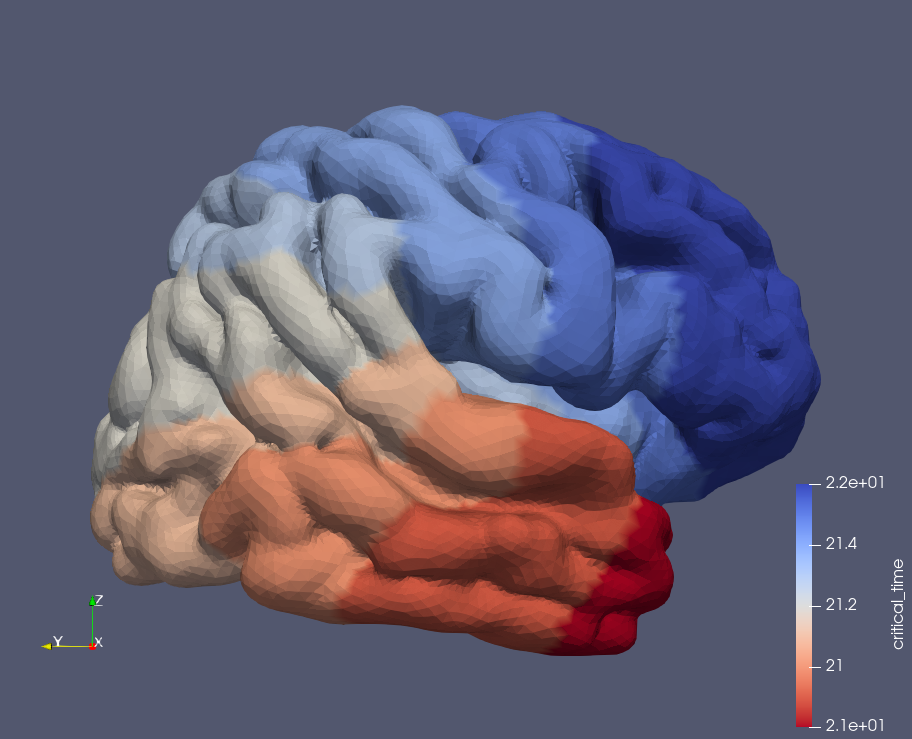
\includegraphics[width=\linewidth]{pics/base.png}
        \caption{Baseline}
    \end{minipage}
    \hfill
    \begin{minipage}{0.4\textwidth}
        \centering
        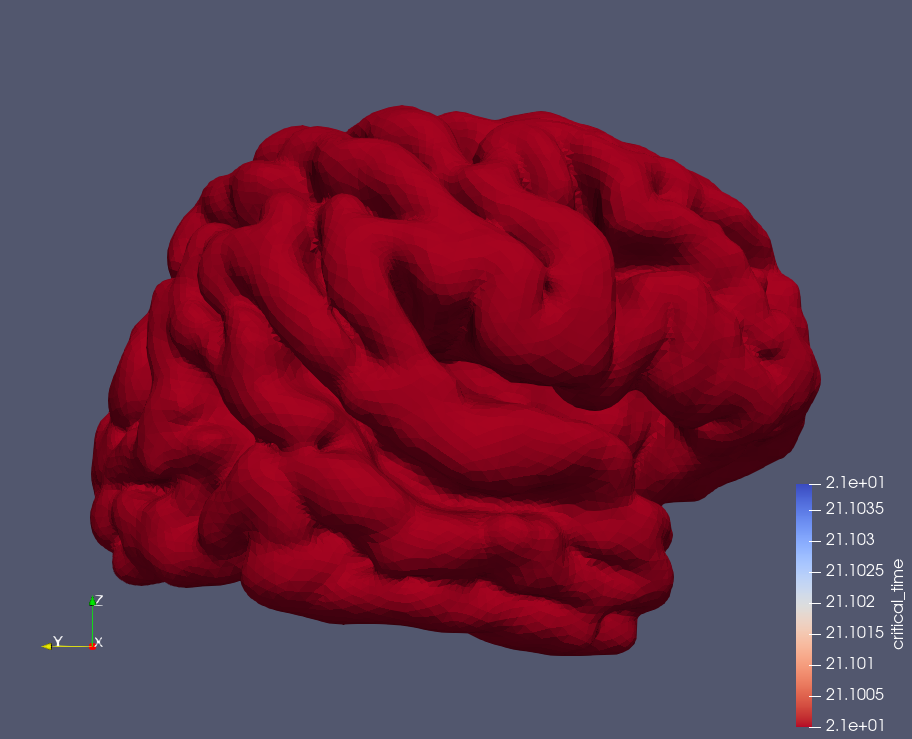
\includegraphics[width=\linewidth]{pics/incdiff.png}
        \caption{Increased diffusion}
    \end{minipage}
    
    \vspace{0.5cm}
    
    % Riga 2
    \begin{minipage}{0.4\textwidth}
        \centering
        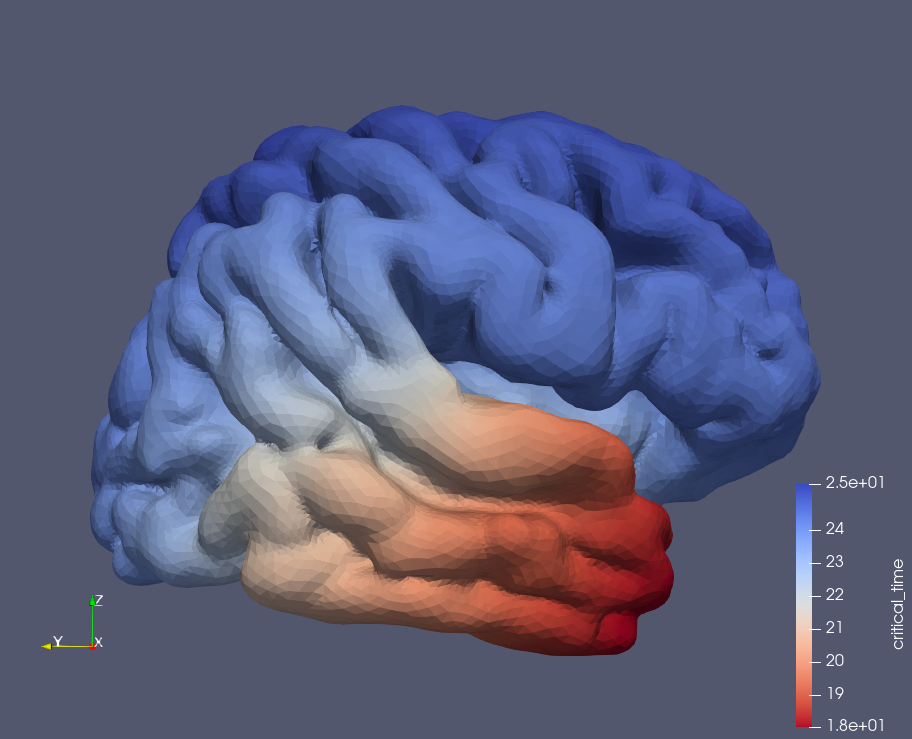
\includegraphics[width=\linewidth]{pics/reddiff.png}
        \caption{Reduced diffusion}
    \end{minipage}
    \hfill
    \begin{minipage}{0.4\textwidth}
        \centering
        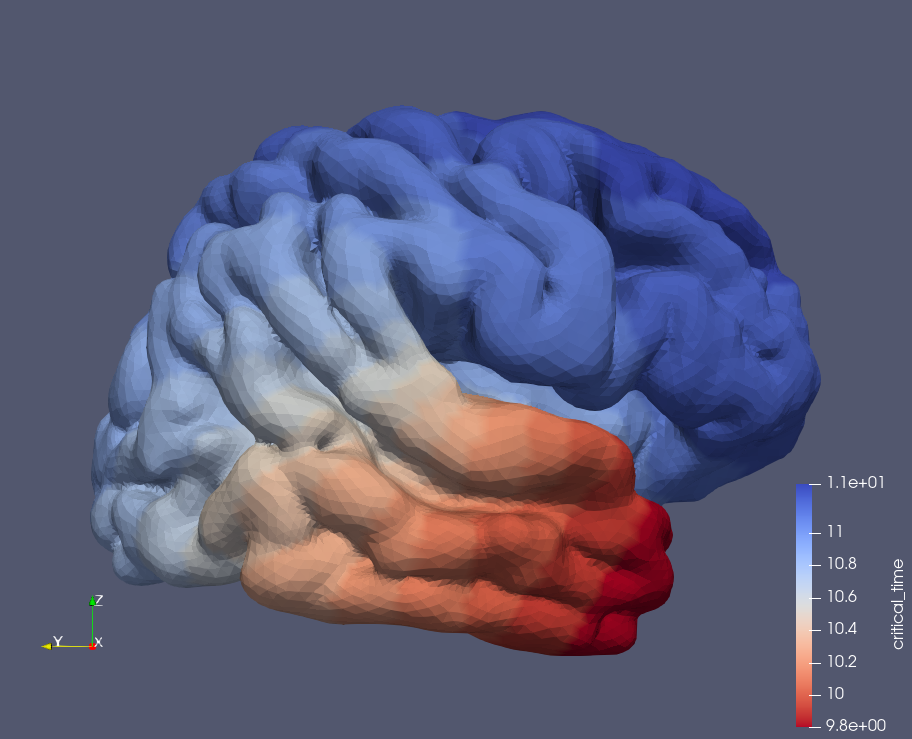
\includegraphics[width=\linewidth]{pics/incgro.png}
        \caption{Increased growth}
    \end{minipage}

\end{figure}

\pagebreak
\section{Results and algorithmic comparison}
% TODO: parallelism
% TODO: comparation between methods
All the algorithms where implemented using Deal.II functions for parallelism.


\noindent An interesting result we obtained from our simulations is that the concentration of proteins in the brain has approximately the same value in each region, so if the protein begins to be harmful at a specific concentration it quickly begins to affect the whole brain in a really short span of time. This correctly predicts the real examples of people affected by neurodegenerative diseases that have a really quick loss of brain functions once the disease begins to show it's signs. The following graph shows the percentage of zones that reached a critical level in the brain. As it can be seen in the graph, the critical threshold is reached with a graph similar to a sigmoid with a really steep slope, indicating a quick degeneration for the disease.
\vspace{1em}

\noindent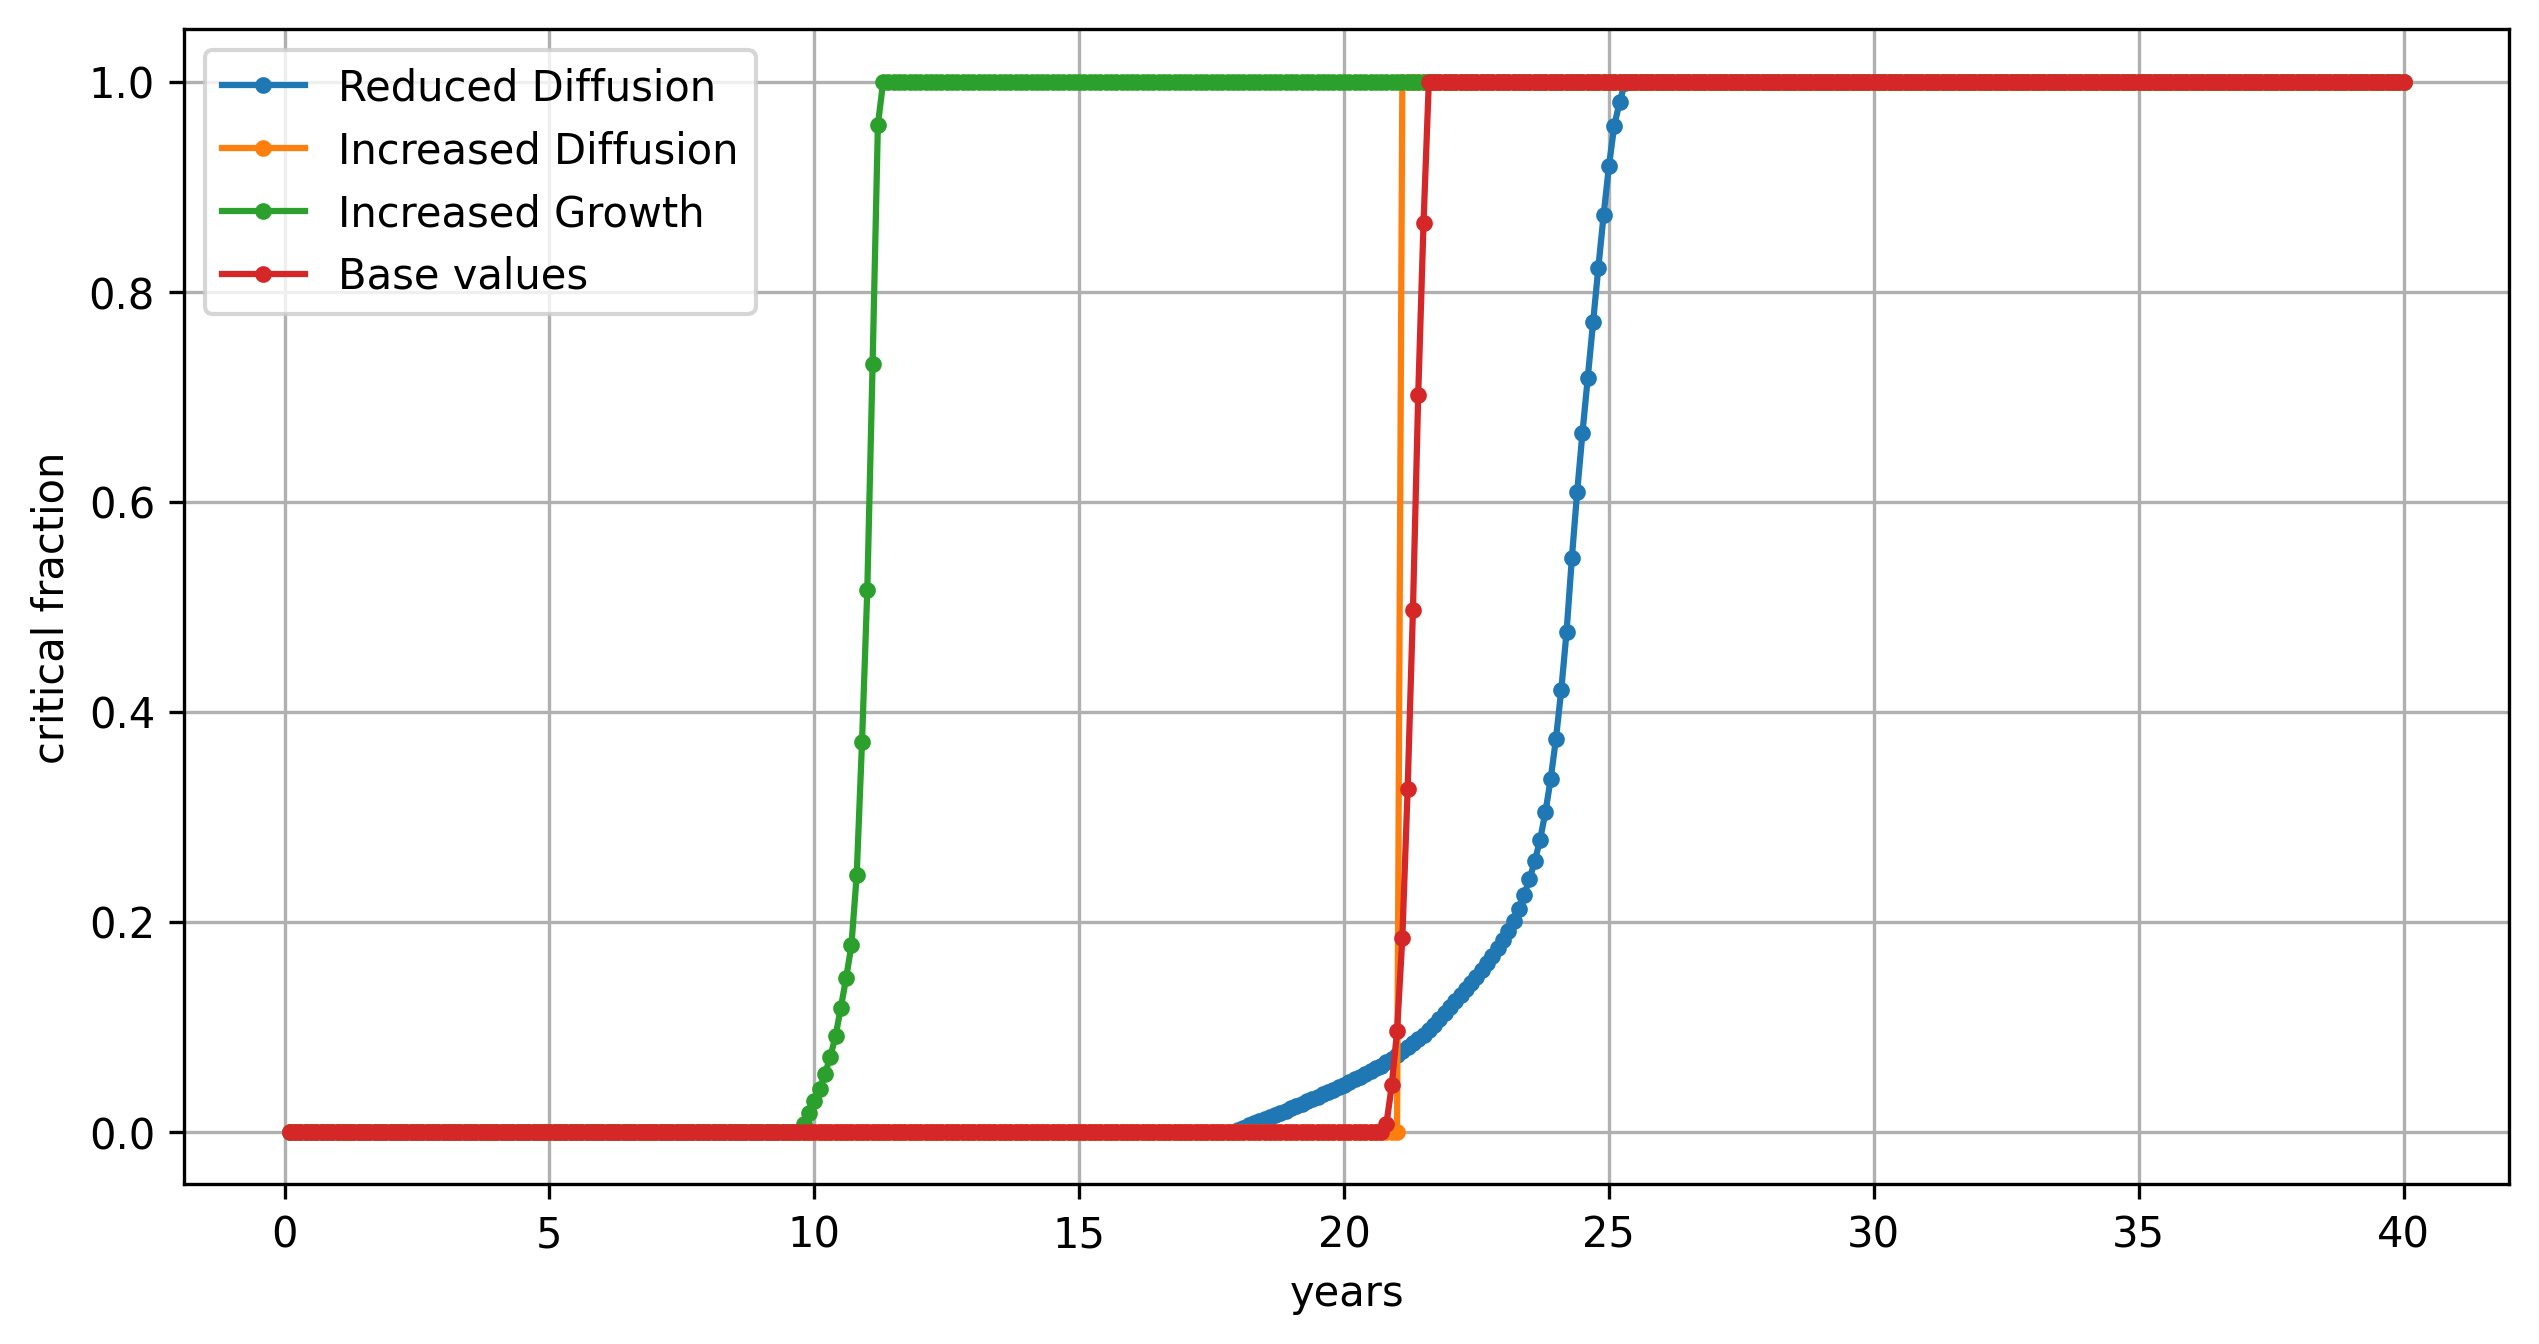
\includegraphics[width=\textwidth]{pics/critical_fraction_comparing.png}

\pagebreak
\subsubsection*{Strong Scalability Test (Implicit Solver)}
A strong scalability test has been done by varying the number of MPI processes and measuring the total execution time.

\noindent The benchmark machine is a laptop running Ubuntu through WSL on Win11 64bit with
    AMD Ryzen 7 6800H (8 physical cores) and
    RAM 16GB. 
    
    

\begin{itemize}
    \item \textbf{Test parameters}: $T = 5 \ \mathrm{years}$, $\Delta t = 0.5$
\end{itemize}

%\begin{center}
%\begin{tabular}{c c}
%\hline
%\textbf{$n_{\mathrm{proc}}$} & \textbf{Time} \\
%\hline
%1 & $6'50''$ \\
%2 & $5'50''$ \\
%4 & $3'22''$ \\
%8 & $2'26''$ \\
%\hline
%\end{tabular}
%\end{center}

\begin{figure}[h!]
    \centering
    \begin{minipage}{0.48\textwidth}
        \includegraphics[width=\linewidth]{pics/ScalabilityTest.png}
    \end{minipage}
    \hfill
    \begin{minipage}{0.48\textwidth}
        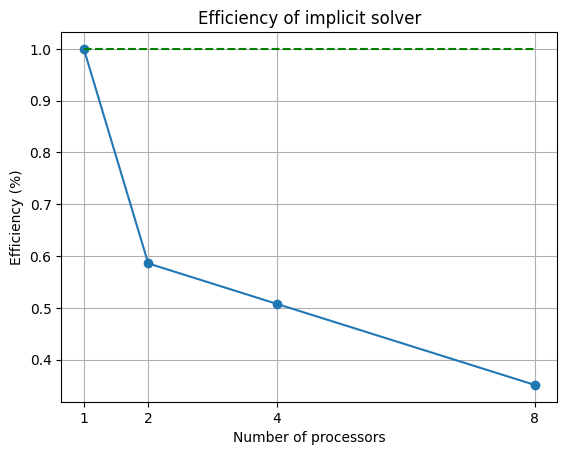
\includegraphics[width=\linewidth]{pics/implicit_efficiency_graph.png}
    \end{minipage}
\end{figure}

% TODO: graph about explosion of disease confirming real evidence
% TODO: say some proteins might act at different percentages of concentration
\pagebreak
\begin{thebibliography}{9}
    \bibitem{diffusion-paper}
    J. Weickenmeier, M. Jucker, A. Goriely, and E. Kuhl. A physics-based model explains the prion-like features of neurodegeneration in Alzheimer’s disease, Parkinson’s disease, and amyotrophic lateral sclerosis. Journal of the Mechanics and
    Physics of Solids, 124:264–281, 2019.
\end{thebibliography}

\end{document}